\documentclass[]{fairmeta}
% Option "twocolumn" available, but please prioritize single-column

\usepackage{graphicx}
\usepackage{amsmath}
\usepackage{amssymb}
\usepackage{booktabs}
\usepackage{adjustbox}
\usepackage{multirow}
\usepackage{arydshln}
\usepackage{colortbl}
\usepackage{overpic}
\usepackage{amsthm}

\usepackage{amsfonts}       % blackboard math symbols
\usepackage{nicefrac}       % compact symbols for 1/2, etc.
\usepackage{microtype}      % microtypography

\usepackage{scalerel}
\newcommand{\sicong}[1]{{\color{blue}#1}}
\usepackage{makecell}

\usepackage{algorithm}
\usepackage{algorithmic}
\usepackage{enumitem}

% define ours package
\usepackage{nicefrac}
\usepackage{multirow}
\usepackage{booktabs}
\usepackage{float}
\usepackage{wrapfig}
\usepackage{bbding}
\usepackage{pifont}
\usepackage{color, colortbl}

\newcommand{\tabincell}[2]{\begin{tabular}{@{}#1@{}}#2\end{tabular}} % \tabincell{c}{
% \newcommand{\hr}[1]{\textcolor{blue}{#1}}
\newcommand{\hr}[1]{\textcolor{black}{#1}}
\definecolor{gray}{gray}{0.9}
\newcommand{\ssymbol}[1]{^{\@fnsymbol{#1}}}
\def\R{\mathbb{R}}
\newcommand{\Lleft}{\left(}
\newcommand{\Rright}{\right)}

\newtheorem{theorem}{Theorem}
\newtheorem{definition}{Definition}
\newtheorem{lemma}{Lemma}
\newtheorem{proposition}{Proposition}

\newcommand{\modelname}{LongVU}

\title{Efficient Track Anything}

\author[1,\dagger]{Yunyang Xiong}
\author[1,2]{Chong Zhou}
\author[1]{Xiaoyu Xiang}
\author[1]{Lemeng Wu}
\author[1]{Chenchen Zhu}
\author[1]{Zechun Liu}
\author[1]{Saksham Suri}
\author[1]{Balakrishnan Varadarajan}
\author[1]{Ramya Akula}
\author[1]{Forrest Iandola}
\author[1,\dagger]{Raghuraman Krishnamoorthi}
\author[1,\dagger]{Bilge Soran}
\author[1,\dagger]{Vikas Chandra}

\affiliation[1]{Meta AI}
\affiliation[2]{Nanyang Technological University}

\contribution[\dagger]{Project lead}

\abstract{Segment Anything Model 2 (SAM 2) has emerged as a powerful tool for video object segmentation and tracking anything. Key components of SAM 2 that drive the impressive video object segmentation performance include a large multistage image encoder for frame feature extraction and a memory mechanism that stores memory contexts from past frames to help current frame segmentation. The high computation complexity of multistage image encoder and memory module has limited its applications in real-world tasks, e.g., video object segmentation on mobile devices. To address this limitation, we propose EfficientTAMs, lightweight track anything models that produce high-quality results with low latency and model size. Our idea is based on revisiting the plain, nonhierarchical Vision Transformer (ViT) as an image encoder for video object segmentation, and introducing an efficient memory module, which reduces the complexity for both frame feature extraction and memory computation for current frame segmentation. We take vanilla lightweight ViTs and efficient memory module to build EfficientTAMs, and train the models on SA-1B and SA-V datasets for video object segmentation and track anything tasks. We evaluate on multiple video segmentation benchmarks including semi-supervised VOS and promptable video segmentation, and find that our proposed EfficientTAM with vanilla ViT perform comparably to SAM 2 model (HieraB+SAM 2) with $\sim$2x speedup on A100 and $\sim$2.4x  parameter reduction. On segment anything image tasks, our EfficientTAMs also perform favorably over original SAM with $\sim$20x  speedup on A100 and $\sim$20x  parameter reduction. On mobile devices such as iPhone 15 Pro Max, our EfficientTAMs can run at $\sim$10 FPS for performing video object segmentation with reasonable quality, highlighting the capability of small models for on-device video object segmentation applications.}

% \date{\today}
\correspondence{\email{yunyang@meta.com}}

\metadata[Project]{\url{https://yformer.github.io/efficient-track-anything/}}

\begin{document}

\maketitle

\section{Introduction}
\label{sec:intro}

\begin{figure*}[t]
\centering
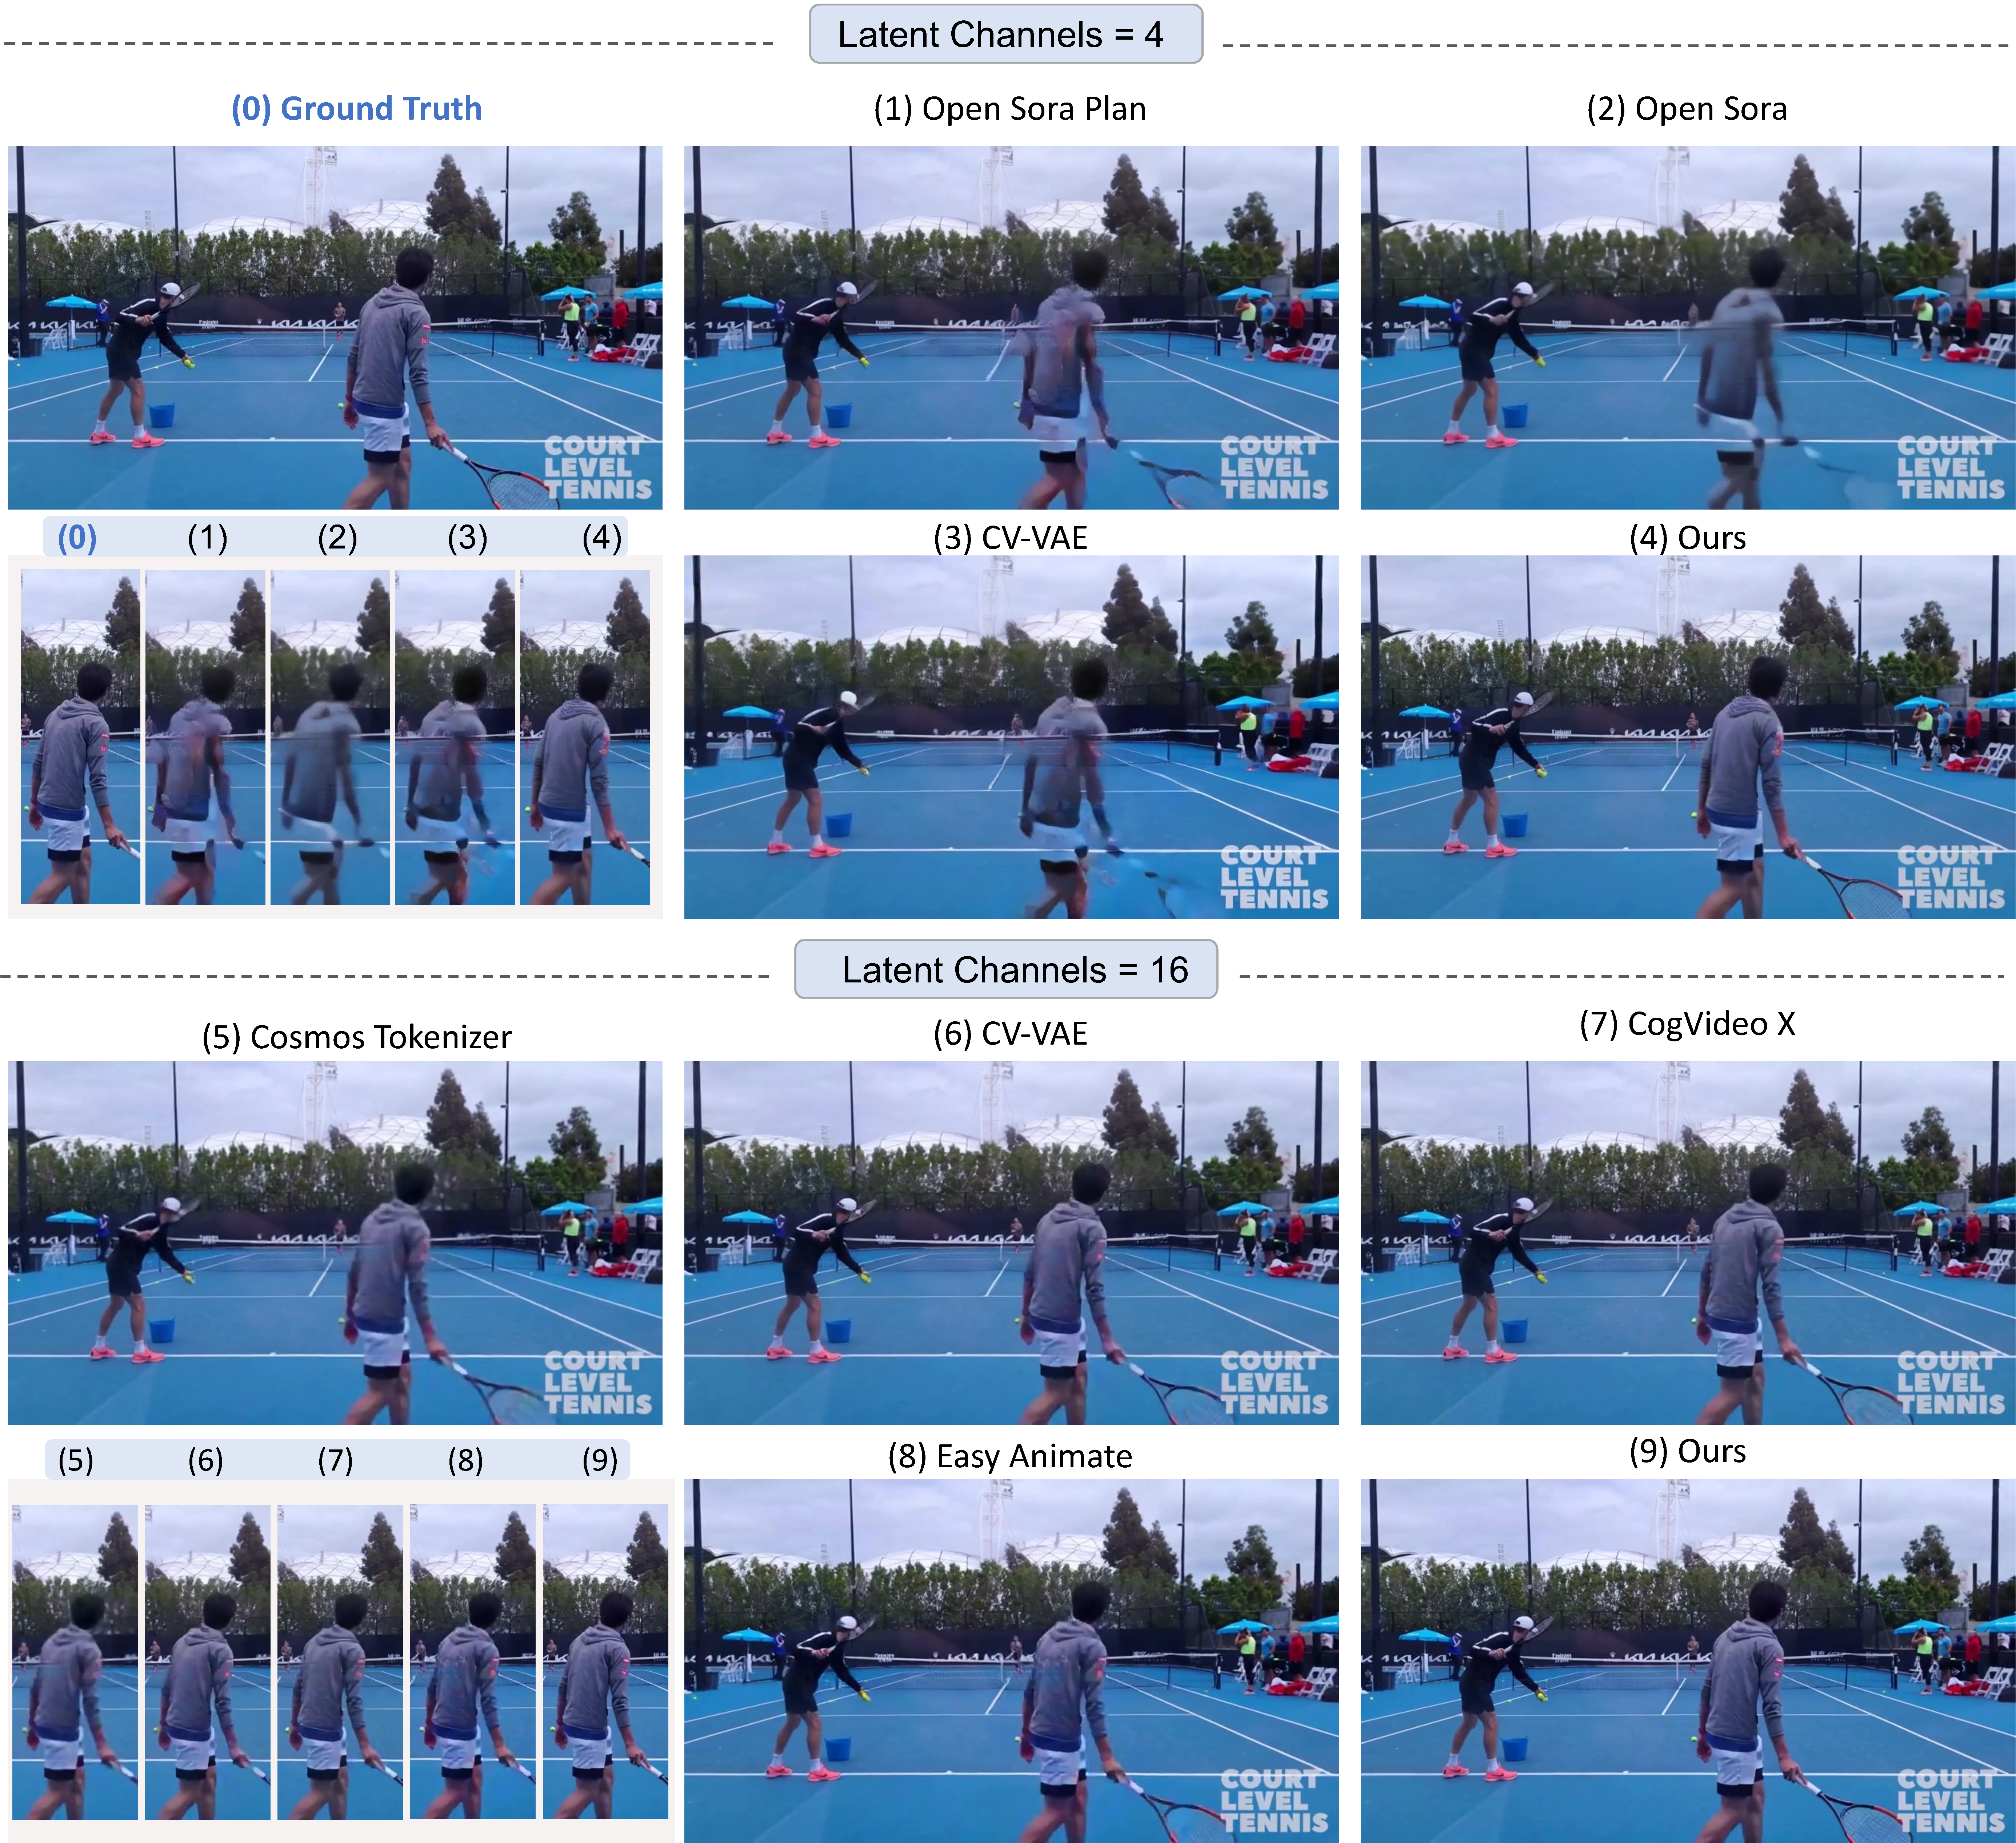
\includegraphics[width=1.0\textwidth]{images/fig1-4and16.pdf}
\caption{
Our reconstruction results compared with a line of three recent strong baseline approaches. 
The ground truth frame is (0). Our model significantly outperforms previous methods, especially under large motion scenarios such as people doing sports.
}
\label{fig:teaser}
\vspace{-3mm}
\end{figure*}



Given the significant attention in the field of video generation, Latent Video Diffusion Models (LVDMs)~\cite{blattmann2023stable, blattmann2023align, he-lvdm, zhou2022magicvideo, he-videocrafter1} have emerged as a popular framework. They have been successfully applied to powerful text-to-video models such as Sora~\cite{videoworldsimulators2024}, VideoCrafter~\cite{he-videocrafter1, chen2024videocrafter2overcomingdatalimitations}, and CogVideoX~\cite{yang2024cogvideox}.
Different from directly generating video pixels, LVDMs generate latent video representations in a compact latent space. This is achieved by first training a Video VAE to encode videos into this latent space.
%
Thus, Video VAE, as a key and fundamental component of LVDMs, has attracted great attention recently.
%
An effective Video VAE can help to reduce the training costs of video diffusion models while improving the final quality of the generated videos.
%
Initially, a series of studies adopt the image VAE from Stable Diffusion~\cite{rombach2022high} for video generation tasks, including AnimateDiff~\cite{guoanimatediff}, MagicVideo~\cite{zhou2022magicvideo}, VideoCrafter1~\cite{he-videocrafter1}, and VideoCrafter2~\cite{chen2024videocrafter2overcomingdatalimitations}. 
%
However, directly adopting an image VAE and compressing video on a frame-by-frame basis leads to temporal flickering due to the lack of temporal correlation. Additionally, the information redundancy along the temporal dimension is not reduced, leading to low training efficiency for subsequent latent video diffusion models.
%
From the introduction of Sora, which compresses videos both temporally and spatially through a Video VAE, a series of studies have emerged that aim to replicate Sora and train their own Video VAEs, including Open Sora~\cite{opensora}, Open Sora Plan~\cite{pku_yuan_lab_and_tuzhan_ai_etc_2024_10948109}, CV-VAE~\cite{zhao2024cv}, CogVideoX~\cite{yang2024cogvideox}, EasyAnimate~\cite{xu2024easyanimatehighperformancelongvideo}, and Cosmos Tokenizer~\cite{cosmos_token}.
%
However, the performance of the current video VAE suffers from many problems, including motion ghost, low-level temporal flickering, blurring (faces, hands, edges, texts), and motion stuttering (lack of correct temporal transition).
% as shown in Fig.~\ref{fig:teaser}.


In this work, we propose a novel cross-modal Video VAE with better spatial and temporal modeling ability in order to solve the aforementioned challenge problems and obtain a robust and high-quality Video VAE.
%
First, we examine different designs for spatial and temporal compression, including simultaneous spatial-temporal (ST) compression and sequential ST compression. 
%
We observed that simultaneous ST compression achieves better low-level temporal smoothness and texture stability, while sequential ST compression achieves better motion recovery, particularly in scenarios of large motion.
%
Thus, we propose a novel architecture that integrates the advantages of both methods and enables effective video detail and motion reconstruction.

Second, we observed that the normally used datasets for text-to-video generation contain text-video pairs. 
Also, during decoding, a text description exists as it serves as the input in the first stage, \textit{i.e.}, the video latent generation stage.
%
To this end, we integrate the text information into the encoding and decoding procedure and propose the first Cross-modal Video VAE.
%
We carefully study how text guidance can be integrated into the spatiotemporal backbone and the mechanism of spatial and temporal semantic guidance. 

In addition, our cross-modal video VAE supports image-video joint training.
To achieve this, we design our network with a fully spatiotemporal factorized architecture, and we feed image and video batches alternately to the network. 
%
During image batches, the data only forwards the spatial part of the network, with the temporal modules being skipped. During video batches, the video forwards both spatial and temporal modules. We also demonstrate that image joint training is crucial for training a video VAE.
%
In summary, our contributions are as follows:
\begin{itemize}
    \item We propose an effective and robust Video VAE, conduct extensive experiments, and achieve the state-of-the-art.
    \item We propose an optimal spatiotemporal modeling approach for Video VAE.
    \item We propose the first cross-modal video VAE that leverages the information from other modalities, i.e., text descriptions, to the best of our knowledge.
    \item Our video VAE is designed and trained to be versatile to conduct both image and video compression. 
\end{itemize}


% \vspace{-2mm}
\section{Related Work}
% \vspace{-2mm}
\label{sec:formatting}
%We now review relevant works on segmentation, vision transformers, and efficient attention.

%-------------------------------------------------------------------------
% \subsection{Video Object Segmentation}
{\bf Video Object Segmentation (VOS)} is a fundamental task in computer vision, segments objects of interest from the background and tracks target objects in a video. 
%Many research works have been proposed in this community on video object segmentation. 
In the unsupervised setting~\citep{grundmann2010efficient,brox2010object,lee2011key,xu2012evaluation,fragkiadaki2012video,perazzi2012saliency,zhang2013video,li2013video,papazoglou2013fast,faktor2014video,wang2015saliency,taylor2015causal,perazzi2016benchmark}, VOS models segment salient objects without a reference mask. In the semi-supervised setting~\citep{pont20172017,xu2018youtube,oh2019video,bhat2020learning,robinson2020learning,li2022recurrent,yang2022decoupling,cheng2022xmem,zhang2023joint,wang2023look,wu2023scalable,cheng2024putting,yang2024scalable}, VOS requires tracking and segmenting objects based on a first-frame mask of target objects. For interactive video object segmentation (iVOS)~\citep{caelles20182018,heo2020interactive,cheng2021modular,homayounfar2021videoclick,yang2023track,cheng2023segment,rajivc2023segment,cheng2024putting,delatolas2024learning}, iVOS models perform object segmentation in videos (masklets) with user guidance, e.g., clicks, bounding boxes, scribbles. In SAM 2~\citep{ravi2024sam}. Semi-supervised VOS and iVOS have been extended to promptable visual segmentation (PVS), where the model can be interactively prompted with different types of inputs such as clicks, boxes, and masks on any frame in a video for segmenting and tracking a valid object.
%-------------------------------------------------------------------------

% \subsection{Vision Transformers}
\noindent {\bf Vision Transformers (ViTs)} have achieved huge success on various vision tasks including image classification~\citep{dosovitskiy2020image}, object detection~\citep{li2022exploring}, image segmentation~\cite{cheng2022masked,kirillov2023segment}, video classification~\citep{fan2021multiscale}, and video object segmentation~\citep{duke2021sstvos,yang2023track}. The original ViT family scales from the efficient ViT-Tiny up to ViT-Huge, with a plain, non-hierarchical architecture. There are also hierarchical vision transformers that combine transformers with hierarchical stage structure, such as Swin~\citep{liu2021swin}, MViT~\citep{fan2021multiscale,li2022mvitv2}, PViT~\citep{wang2021pyramid}, and Hiera~\citep{ryali2023hiera}. While being successful, hierarchical models are usually slower than their plain ViT counterparts for practical deployment~\citep{ryali2023hiera}. 
Combining ViT with convolutions~\citep{lecun1989backpropagation} has been explored for fast hybrid models such as MobileViT~\citep{mehta2021mobilevit}, LeViT~\citep{graham2021levit},  EfficientFormer\citep{li2022efficientformer}, Next-ViT\citep{li2022next}, Tiny-ViT\citep{wu2022tinyvit}, Castling-ViT\citep{you2023castling}, EfficientViT~\citep{liu2023efficientvit}, and MobileNetv4~\citep{qin2024mobilenetv4}. This line of progression towards building efficient ViTs is orthogonal to our
EfficientTAM work towards building efficient video object segmentation. Following SAM~\citep{kirillov2023segment} and EfficientSAMs~\citep{xiong2024efficientsam}, we are pursuing plain ViT backbones for efficient video object segmentation and track anything tasks.  
%The community has also shown increasing interest in efficient vision transformers; \citep{touvron2021training} presented smaller ViTs such as ViT-Small and ViT-Tiny for complementing ViT-Huge, ViT-Large, and ViT-Base in \citep{dosovitskiy2020image}. 


%-------------------------------------------------------------------------
% \subsection{Efficient Attention}
\noindent {\bf Efficient Attention.} The field has developed methods to reduce the quadratic cost of standard self-attention with respect to input sequence length~\cite{attention_is_all_you_need}. 
Local windowed attention has been applied in \cite{beltagy2020longformer,zaheer2020bigbird} for reducing the complexity of self-attention. In \cite{shen2018efficient,katharopoulos-et-al-2020}, a linear dot product approximation is proposed to linearize the softmax matrix in self-attention by heuristically separating keys and queries. In \cite{choromanski2020rethinking}, the Performer model uses random features to approximate self-attention, achieving linear time and memory cost. Nystr\"{o}mformer in \cite{xiong2021nystromformer} makes use of the Nystr\"{o}m method to approximate self-attention with a linear cost. Linformer \cite{wang2020linformer} shows that self-attention is low-rank, which can be approximated by learning linear projection matrices for the keys and values. The approach of~\citep{liu2023efficientvit,you2023castling} leverages the associative property of matrix multiplication for efficient attentions in vision transformers. This direction has shown success and has achieved decent performance on vision tasks. However, in preliminary experiments we found that these methods underperformed in a memory cross-attention module when adapted for efficiency improvement.


%-------------------------------------------------------------------------
% \subsection{Segment Anything Model}
\noindent {\bf Segment Anything Model.} SAM~\citep{kirillov2023segment} is a vision foundation model that can segment any object in an image using interactive prompts such as points and bounding boxes. SAM has demonstrated remarkable zero-shot transfer performance and high versatility for many vision tasks including a broad range of segmentation applications~\citep{chen2023semantic,cen2023sad,deng2023segment,chen2023sam}, in-painting~\citep{yu2023inpaint}, image restoration~\citep{jiang2023restore}, image editing~\citep{gao2023editanything}, image shadow removal~\citep{zhang2023deshadow}, medical image segmentation~\citep{ma2023segment}, camouflaged object detection~\citep{tang2023can}, transparent object detection~\citep{han2023segment}, concept-based explanation~\citep{sun2023explain}, semantic communication~\citep{tariq2023segment}, and object tracking~\citep{cheng2023segment,yang2023track}. The strong ability on image segmentation with flexible prompts motivates the extension of SAM for video object segmentation and track anything. Track Anything Model (TAM)~\citep{yang2023track} combines SAM and XMem~\cite{cheng2022xmem} for interactive video object tracking and segmentation with SAM for frame segmentation and XMem for tracking. SAM-Track~\citep{cheng2023segment} perform object tracking and segmentation in videos by combining SAM~\citep{kirillov2023segment}, DeAOT~\citep{yang2022decoupling}, and Grounding-Dino~\citep{liu2023grounding}. The latest SAM 2~\citep{ravi2024sam} extended SAM for video segmentation through a hierarchical image encoder for frame embeddings and a memory module that conditions current frame embeddings on past frames. Motivated by mobile app use-cases and computationally-constrained applications, recent works have reduced the computational cost of SAM, such as MobileSAM~\citep{zhang2023faster}, FastSAM~\citep{zhao2023fast}, and EfficientSAM~\citep{xiong2024efficientsam}.
The present paper focuses on improving the efficiency challenges of SAM 2 for practical deployment of video object segmentation and track anything.  
\section{Method}
\label{sec:method}

\subsection{Practical choice of diffusion paradigm}
\label{subsec:practical_dwm}

Building on the background provided in Section \ref{sec:framework}, we now introduce \textsc{diamond} as a practical realization of a diffusion-based world model. In particular, we now define the drift and diffusion coefficients $\mathbf{f}$ and $g$ introduced in Section \ref{subsec:diffusion}, corresponding to a particular choice of diffusion paradigm. While \textsc{ddpm} \citep{ho2020DDPM} is an example of one such choice (as described in Appendix \ref{app:ddpm}) and would historically be the natural candidate, we instead build upon the \textsc{edm} formulation proposed in \citet{karras2022elucidating}. The practical implications of this choice are discussed in Section \ref{subsec:diffusion_choice}. In what follows, we describe how we adapt \textsc{edm} to build our diffusion-based world model.

We consider the perturbation kernel $p^{0\tau}(\x_{t+1}^\tau \mid \x_{t+1}^0) = \mathcal{N}(\x_{t+1}^\tau; \x_{t+1}^0, \sigma^2(\tau) \mathbf{I})$, where $\sigma(\tau)$ is a real-valued function of diffusion time called the noise schedule. This corresponds to setting the drift and diffusion coefficients to $\mathbf{f}(\x, \tau) = \mathbf{0}$ (affine) and $g(\tau) = \sqrt{2 \dot \sigma(\tau) \sigma(\tau)}$.

We use the network preconditioning introduced by \citet{karras2022elucidating} and so parameterize $\mathbf{D}_\theta$ in Equation \ref{eq:denoising_sm_conditional} as the weighted sum of the noised observation and the prediction of a neural network $\mathbf{F}_\theta$,
\begin{equation}
\label{eq:karras_wrappers} 
    \mathbf{D}_\theta(\x_{t+1}^\tau, y_t^\tau) = c_\text{skip}^\tau \; \x_{t+1}^\tau + c_\text{out}^\tau \; \mathbf{F}_\theta \big( c_\text{in}^\tau \; \x_{t+1}^\tau, y_t^\tau \big),
\end{equation}
where for brevity we define $y_t^\tau \coloneqq (c_\text{noise}^\tau, \x^0_{\le t}, a_{\le t})$ to include all conditioning variables.

The preconditioners $c_\text{in}^\tau$ and $c_\text{out}^\tau$ are selected to keep the network's input and output at unit variance for any noise level $\sigma(\tau)$, $c_\text{noise}^\tau$ is an empirical transformation of the noise level, and $c_\text{skip}^\tau$ is given in terms of $\sigma(\tau)$ and the standard deviation of the data distribution $\sigma_\text{data}$, as $c_{skip}^\tau = \sigma_{data}^2/(\sigma_{data}^2 + \sigma^2(\tau))$. These preconditioners are fully described in Appendix \ref{appendix:karras_conditioners}.

Combining Equations \ref{eq:denoising_sm_conditional} and \ref{eq:karras_wrappers} provides insight into the training objective of $\mathbf{F}_\theta$,
\begin{align}
\label{eq:effective_obj}
\mathcal{L}(\theta)  = \bbe \Big[ \Vert 
\underbrace{\mathbf{F}_\theta \big( c_\text{in}^\tau \x_{t+1}^\tau, y_t^\tau \big)}_\text{Network prediction} - 
\underbrace{\frac{1}{c_\text{out}^\tau} \big( \x_{t+1}^0 - c_\text{skip}^\tau \x_{t+1}^\tau\big)}_\text{Network training target}
\Vert^2 \Big].
\end{align}
The network training target adaptively mixes signal and noise depending on the degradation level $\sigma(\tau)$.
When $\sigma(\tau) \gg \sigma_\text{data}$, we have $c_\text{skip}^\tau \to 0$, and the training target for $\mathbf{F}_\theta$ is dominated by the clean signal $\x_{t+1}^0$. Conversely, when the noise level is low, $\sigma(\tau) \to 0$, we have $c_\text{skip}^\tau \to 1$, and the target becomes the difference between the clean and the perturbed signal, i.e. the added Gaussian noise. Intuitively, this prevents the training objective to become trivial in the low-noise regime. In practice, this objective is high variance at the extremes of the noise schedule, so \citet{karras2022elucidating} sample the noise level $\sigma(\tau)$ from an empirically chosen log-normal distribution in order to concentrate the training around medium-noise regions, as described in Appendix \ref{appendix:karras_conditioners}.

We use a standard U-Net 2D for the vector field $\mathbf{F}_\theta$ \citep{ronneberger2015unet}, and we keep a buffer of $L$ past observations and actions that we use to condition the model. We concatenate these past observations to the next noisy observation channel-wise, and we input actions through adaptive group normalization layers \citep{adagn} in the residual blocks \citep{He2015} of the U-Net.

As discussed in Section \ref{subsec:dwm_training} and Appendix \ref{appendix:sampling}, there are many possible sampling methods to generate the next observation from the trained diffusion model. While our codebase supports a variety of sampling schemes, we found Euler's method to be effective without incurring the cost of additional NFE required by higher order samplers, or the unnecessary complexity of stochastic sampling.

\subsection{Reinforcement learning in imagination}
\label{subsec:rl}

Given the diffusion model from Section \ref{subsec:practical_dwm}, we now complete our world model with a reward and termination model, required for training an RL agent in imagination. Since estimating the reward and termination are scalar prediction problems, we use a separate model $R_\psi$ consisting of standard \textsc{cnn} \citep{cnn_lecun,He2015} and \textsc{lstm} \citep{lstm,Gers2000} layers to handle partial observability. The RL agent involves an actor-critic network parameterized by a shared \textsc{cnn-lstm} with policy and value heads. The policy $\pi_\phi$ is trained with \textsc{reinforce} with a value baseline, and we use a Bellman error with $\lambda$-returns to train the value network $V_\phi$, similar to \citet{iris2023}. We train the agent entirely in imagination as described in Section \ref{subsec:pomdp_and_wm}. The agent only interacts with the real environment for data collection. After each collection stage, the current world model is updated by training on all data collected so far. Then, the agent is trained with RL in the updated world model environment, and these steps are repeated. This procedure is detailed in Algorithm \ref{alg:diamond}, and is similar to \citet{kaiser2019atari100k,hafner2020dream,iris2023}. We provide architecture details, hyperparameters, and RL objectives in Appendices \ref{app:architectures}, \ref{app:hyperparams}, \ref{appendix:rl_actor_critic}, respectively.

\section{Experiments}
\subsection{Experimental Setting}
\noindent \textbf{Pretraining.} The SA-1B dataset  consists of 11M diverse, high resolution images with 1.1B high-quality segmentation masks. Similar to~\citep{ravi2024sam}, we pretrain our EfficientTAM without memory components on SA-1B dataset~\citep{kirillov2023segment} for 90k steps. Our ViT image encoder is initialized from pre-trained ViTs~\citep{xiong2024efficientsam}
. We use the AdamW optimizer ~\citep{loshchilov2017decoupled} with a momentum, ($\beta_1 = 0.9$, $\beta_2 = 0.999$), a global batch size of 256, and a initial learning rate of $4e-4$. The learning rate is decayed by a reciprocal square root learning rate schedule~\citep{zhai2022scaling} with 1k iterations linear warmup and 5k iterations linear cooldown. We set weight decay to 0.1. We do not apply drop path for our image encoder. Layer-wise decay~\citep{clark2020electra} is set to 0.8. We apply horizontal flip augmentation and resize the input image resolution to $1024\times 1024$. We restrict our training to $64$ masks per image. Our models are pre-trained on 256 A100 GPUs with 80GB GPU memory with a linear combination of focal and dice loss for mask prediction (e.g., a ratio of 20:1). Bfloat16 is used during the training.

\noindent \textbf{Full Training Datasets.} Following~\citep{ravi2024sam}, we train our EfficientTAM including memory components on SA-V dataset~\citep{ravi2024sam} and a 10\% subset of SA-1B~\citep{kirillov2023segment}. SA-V is a large-scale and diverse video segmentation dataset, including 51K videos captured across 47 countries and 600K mask annotations covering whole objects and parts. SA-V video resolution ranges from 240p to 4K and duration ranges from 4 seconds to 138 seconds. Unlike SAM 2, we do not use other open-source datasets or internal datasets during our training for a fair comparison with baselines. 

\noindent \textbf{Full Training Implementation Details.} Similar to  ~\citep{ravi2024sam}, we train our EfficientTAM for 300k steps after pretraining. We use the AdamW optimizer ~\citep{loshchilov2017decoupled} with a momentum, ($\beta_1 = 0.9$, $\beta_2 = 0.999$), a batch size of 256, and a initial learning rate of $6e-5$ for image encoder and $3e-4$ for other components of the model. The learning rate is decayed by a cosine schedule with 15k iterations linear warmup. We set weight decay to 0.1. We do not apply drop path for our image encoder. Layer-wise decay~\citep{clark2020electra} is set to 0.8. We apply horizontal flip image augmentation and resize the input image resolution to $1024\times 1024$. For video, we apply horizontal flip augmentation, affine transformation with degree $25$ and shear $20$, color jittering with brightness $0.1$, contrast $0.03$, saturation $0.03$, gray scale augmentation with a probability of $0.05$, We restrict our training to $64$ masks per image and $3$ masks per frame for video. Our models are trained on 256 A100-80G GPUs with a linear combination of focal and dice losses for mask prediction, mean-absolution-error loss for IoU prediction, and cross-entropy loss for object prediction. The ratio for the linear combination loss is 20:1:1:1. Bfloat16 is used for training.

\noindent \textbf{Downstream Tasks/Datasets/Models.} \underline{\textit{Tasks and Datasets.}} We consider zero-shot video tasks including promptable video segmentation and semi-supervised video object segmentation, and zero-shot image tasks to demonstrate the competing capabilities of EfficientTAM on image and video segmentation.
For zero-shot image tasks, we evaluate EfficientTAM on 37 datasets including 23 datasets of SA-23~\citep{kirillov2023segment} and 14 video datasets introduced in~\citep{ravi2024sam}. For zero-shot video tasks, we evaluate our EfficientTAM on 9 densely annotated datasets for promptable video segmentation. We use 17 video datasets to evaluate zero-shot accuracy under interactive semi-supervised VOS setting using different prompts. For the standard semi-supervised VOS setting where a ground-truth mask on the first frame is provided, MOSE~\citep{ding2023mose}, DAVIS2017~\citep{pont20172017}, LVOS~\citep{hong2024lvos}, SA-V~\citep{ravi2024sam}, and YTVOS~\citep{xu2018youtube} are used to measure the VOS accuracy. We refer readers to~\citep{kirillov2023segment,ravi2024sam} for the details of these datasets.
\underline{\textit{Models.}} We use our EfficientTAM for zero-shot image and video tasks.

\noindent\textbf{Baselines and Evaluation Metrics.}
\underline{\textit{Baselines.}} For the standard semi-supervised VOS task, where the first-frame mask is provided, we compare the performance of our EfficientTAM with SAM 2\citep{ravi2024sam}, Cutie-base\citep{cheng2024putting}, DEVA~\citep{cheng2023tracking}, XMem~\citep{cheng2022xmem}, etc.
For the zero-shot promptable video segmentation task and the interactive semi-supervised video object segmentation task using different prompts, we compare our method with SAM2~\citep{ravi2024sam}, SAM+XMem++~\citep{ravi2024sam}, and SAM+Cutie~\citep{ravi2024sam}. For zero-shot image segmentation task, we compare with SAM~\citep{kirillov2023segment} and SAM2~\citep{ravi2024sam}. Note that we use the opensource version of SAM 2 (without training on MOSE/LVOS/YTVOS) for comparison. We also acknowledge the very recent release of SAM 2.1 trained with long memory contexts. 
\underline{\textit{Evaluation Metrics.}} We evaluate our method and all baselines using the accuracy metrics of the combined $\mathcal{J}$(region similarity)\&$\mathcal{F}$(contour accuracy),  for zero-shot video segmentation tasks; mIoU (mean intersection over union) for zero-shot image segmentation tasks. For efficiency metrics, we compare the number of model parameters or inference throughput on GPU (e.g, A100) and latency on mobile devices (e.g., iPhone 15 Pro Max). We follow SAM 2~\citep{ravi2024sam} to report metrics. When providing main results on MOSE, LVOS and YTVOS, we submit to their benchmarking servers to evaluate on, \textit{MOSE val}, \textit{LVOS val}, and \textit{YTVOS2019 val}, for final performance. For ablation studies, we evaluate on a MOSE development set, \textit{MOSE dev} with 200 randomly-sampled videos from the MOSE training split~\citep{ravi2024sam}.

\subsection{Main Results}
% Please add the following required packages to your document preamble:
% \usepackage{multirow}
% Please add the following required packages to your document preamble:
% \usepackage{multirow}
\begin{table*}[t]
% \vspace{-3mm}
\centering
\resizebox{0.9\linewidth}{!}{
\begin{tabular}{c|cccc|c|c|c|c}
\hline
\multirow{2}{*}{Method}                                   & \multicolumn{4}{c|}{$\mathcal{J}$\&$\mathcal{F}$}                                                                                                                                                         & $\mathcal{G}$                                            & \multirow{2}{*}{\begin{tabular}[c]{@{}c@{}}\\Parameters\\ (M)\end{tabular}} & FPS   & Latency (ms) \\ \cline{2-6} \cline{8-9} 
                                                          & \begin{tabular}[c]{@{}c@{}}MOSE \\ val\end{tabular} & \begin{tabular}[c]{@{}c@{}}DAVIS\\ 2017 val\end{tabular} & \begin{tabular}[c]{@{}c@{}}LVOS\\ val\end{tabular} & \begin{tabular}[c]{@{}c@{}}SA-V\\ test\end{tabular} & \begin{tabular}[c]{@{}c@{}}YTVOS\\ 2019 val\end{tabular} &                                                                           & A100  & iPhone15     \\ \hline
STCN~\citep{cheng2021rethinking}                                                      & 52.5                                                & 85.4                                                     & -                                                  & 57.3                                                & 82.7                                                     &   54                                                                        & 62.8  & -            \\
% R50-AOT-L~\citep{yang2021associating}                                                 & 58.4                                                & 84.9                                                     & -                                                  & 56.7                                                & 85.3                                                     & 15                                                                          & 6.4   & -            \\
% DeAOT-R50~\citep{yang2022decoupling}                                                 & 64.1                                                & 86.0                                                     & -                                                  & 59.9                                                & 85.3                                                     &                                                              20             & 11.7  & -            \\
RDE~\citep{li2022recurrent}                                                       & 46.8                                                & 84.2                                                     & -                                                  & 48.4                                                & 81.9                                                     &      64                                                                     & 88.8  & -            \\
XMem~\citep{cheng2022xmem}                                                      & 59.6                                                & 86.0                                                     & -                                                  & 60.1                                                & 85.6                                                     &     62                                                                      & 61.2  & -            \\
% SimVOS-B~\citep{wu2023scalable}                                                 & -                                                   & 88.0                                                     & -                                                  & 41.2                                                & 84.2                                                     &                                                                           & 3.3   & -            \\
% JointFormer~\citep{zhang2023joint}                                               & -                                                   & 90.1                                                     & -                                                  & -                                                   & 87.4                                                     &                                                                           & 3.0   & -            \\
% ISVOS~\citep{wang2023look}                                                     & -                                                   & 88.2                                                     & -                                                  & -                                                   & 86.3                                                     &                                                                           & 5.8   & -            \\
DEVA~\citep{cheng2023tracking}                                                      & 66.0                                                & 87.0                                                     & 55.9                                               & 53.8                                                & 85.4                                                     &      69                                                                     & 65.2  & -            \\
Cutie-base~\citep{cheng2024putting}                                                & 69.9                                                & 87.9                                                     & 66.0                                               & 61.6                                                & 87.0                                                     & 35                                                                        & 65    & -            \\
Cutie-base+~\citep{cheng2024putting}                                               & 71.7                                                & 88.1                                                     & -                                                  & 62.3                                                & 87.5                                                     & 35                                                                        & 57.2  & -            \\
SAM 2~\citep{ravi2024sam}                                                     & 72.8                                                & 88.9                                                     &             76.2                                       &         74.7                                        & 87.9                                                     & 81                                                                        & 43.8  & -            \\ \hline
\rowcolor{gray} EfficientTAM-Ti/2 (ours) & 68.4                                                & 88.4                                                     & 66.1                                               & 70.8                                                & 87.1                                                     & 18                                                                        & 109.4 & 261.4        \\
\rowcolor{gray} EfficientTAM-Ti (ours)   & 69.3                                                & 89.1                                                     & 69.6                                               & 70.7                                                & 86.7                                                     & 18                                                                        & 96.2  & 840.5        \\
\rowcolor{gray} EfficientTAM-S/2 (ours)  & 70.8                                                & 88.6                                                     & 72.1                                               & 74.0                                                & 87.2                                                     & 34                                                                        & 109.4 & 450          \\
\rowcolor{gray} EfficientTAM-S (ours)    & 71.4                                                & 89.2                                                     & 73.4                                               & 74.5                                                & 87.2                                                     & 34                                                                        & 85.0  & 1010.8       \\ \hline
\end{tabular}}
\caption{Standard semi-supervised video object segmentation results across video object segmentation benchmarks.}
\label{tab:vos}
\end{table*}
\textbf{Standard Semi-Supervised Video Object Segmentation.} Semi-supervised video object segmentation is the process of object segmentation and tracking in a video based on a ground-truth mask on the first frame. We follow SAM 2~\citep{ravi2024sam} and report accuracy of our methods on this standard semi-supervised video object segmentation task. We also report latency on a single A100 GPU with a batch size of 1. We evaluate EfficientTAMs with different image encoders, ViT-Tiny and ViT-Small, and memory modules, original memory block and efficient memory block with a $2\times2$ window pooling for a trade-off between efficiency and accuracy. EfficientTAM-S denotes EfficientTAM using a ViT-Small image encoder and the original memory block, and EfficientTAM-S/2 denotes EfficientTAM with a ViT-Small image encoder and efficiency memory block with a $2\times 2$ window pooling. \cref{tab:vos} compares our EfficientTAM with VOS baselines including SAM 2~\citep{ravi2024sam}, Cutie-base~\citep{cheng2024putting}, and XMem~\citep{cheng2022xmem}. On SA-V test, our EfficientTAM-S achieves 74.5 $\mathcal{J}$\&$\mathcal{F}$, outperforming Cutie-base, Cutie-base+, and XMem by 12.2, 12.9, and 14.4, respectively. On long-term video object segmentation benchmark, LVOS, we can also see that Our EfficientTAM-S outperform Cutie-base and XMem by a large margin. Notice that our EfficientTAM-S only underperforms SAM 2 by $<2$ $\mathcal{J}$\&$\mathcal{F}$ or $\mathcal{G}$ across 5 video benchmarks with $\sim$2x speedup and $\sim$2.4x fewer parameters. Further, EfficientTAM with efficient memory attention performs slightly worse than the one with original memory attention, but with much speedup, especially on mobile devices, $>$2x reduced latency on iPhone 15. For example, EfficientSAM-S achieves 74.5 $\mathcal{J}$\&$\mathcal{F}$ on SA-V test with 1010.8 ms running time per frame on iPhone 15. EfficientSAM-S/2 with efficient cross-memory attention obtain 74.0 $\mathcal{J}$\&$\mathcal{F}$ with only 450 ms. These results show the extraordinary benefits of EfficientTAMs for semi-supervised video object segmentation and validate the advantages of our methods for practical deployment.

\begin{figure*}[t]
    \centering
    \begin{overpic}[width=0.4\linewidth]{figures/offline_full.pdf}
    \end{overpic}
    \begin{overpic}[width=0.4\linewidth]{figures/online_full.pdf}
    \end{overpic}
    \caption{Promptable video segmentation results across 9 video segmentation datasets under interactive offline (left) and online (right) evaluation settings. The average $\mathcal{J}$\&$\mathcal{F}$ over $1, \dots, 8$ interacted frames is reported.}
    \label{fig:pvs}
\end{figure*}

\begin{figure*}[h]
\centering
% \vspace{5pt}
\begin{overpic}[width=0.85\linewidth]{figures/video_seg_track_2.png}
\put (-8.3,25) {\scriptsize{SAM 2}}
\put (-12.0,18) {\scriptsize{EfficientTAM}}
\put (-8.3,10) {\scriptsize{SAM 2}}
\put (-12.0,3) {\scriptsize{EfficientTAM}}
\end{overpic}
\caption{Visualization results on video segmentation and tracking with SAM 2, and our EfficientTAM model. We sampled a subset of frames for visualization. The segmented objects, e.g., the goose and the camel, are colored in red. }
\label{fig:visual_vost}
\end{figure*}


\noindent \textbf{Promptable Video Segmentation.} Similar to SAM 2~\citep{ravi2024sam}, we evaluate promptable video segmentation using two settings, offline evaluation and online evaluation. For offline evaluation, we make multiple passes through a video to annotate frames  w.r.t. the largest model error. For online evaluation, we make a single pass through the video to annotate frames. 3 clicks per frame are used for the evaluations on 9 densely annotated video datasets including 
EndoVis, ESD, LVOSv2, LV-VIS, UVO, VOST, PUMaVOS, Virtual KITTI 2, and VIPSeg. Average $\mathcal{J}$\&$\mathcal{F}$ accuracy over $1, \dots, 8$ interacted frames is reported. \cref{fig:pvs} shows the comparison between our method and strong baselines including SAM 2, SAM + XMem++, and SAM + Cutie. EfficientTAM outperforms SAM + XMem++ and SAM + Cutie for both evaluation settings. EfficientTAM also reduces the gap between SAM 2 for offline and online settings. Specifically, with 8 annotated frames with 3-click, EfficientTAM-S and EfficientTAM-S/2 achieve $\sim$ 82 $\mathcal{J}$\&$\mathcal{F}$ in average for offline evaluation setting and $\sim$ 81 $\mathcal{J}$\&$\mathcal{F}$ in average for online evaluation, outperforming SAM + XMem++, and SAM + Cutie by $>$3 $\mathcal{J}$\&$\mathcal{F}$ and reducing the gap of SAM 2. This set of experiments further validate the effectiveness of our EfficientTAM on promptable video segmentation. 

\begin{table}[t]
    \centering
    \resizebox{0.8\linewidth}{!}{
    \begin{tabular}{c|ccccc}
    \hline
    Method           & 1-click & 3-click & 5-click & bounding box & ground-truth mask \\ \hline
    SAM+XMem++       & 56.9    & 68.4    & 70.6    & 67.6         & 72.7              \\
    SAM+Cutie        & 56.7    & 70.1    & 72.2    & 69.4         & 74.1              \\
    SAM 2            & 64.3    & 73.2    & 75.4    & 72.9         & 77.6              \\ \hline
    \rowcolor{gray} EfficientTAM-S/2 & 60.5    & 72.8    & 75.4    & 71.2         & 76.8              \\
    \rowcolor{gray} EfficientTAM-S   & 63      & 74.1    & 75.7    & 73.2         & 77.8              \\ \hline
    \end{tabular}}
    \caption{Interactive semi-supervised video object segmentation results with different prompts. We report averaged $\mathcal{J}$\&$\mathcal{F}$ zero-shot accuracy across 17 video datasets for each type of prompt.}
    \label{tab:interactive}
\end{table}
\noindent \textbf{Interactive Semi-Supervised Video Object Segmentation.} We also evaluate our method on the interactive semi-supervised video object segmentation task with click, box, or mask prompts provided only on the first frame by following SAM 2. In \cref{tab:interactive}, we report the average $\mathcal{J}$\&$\mathcal{F}$ accuracy over 17 video datasets for each type of prompt. We observe that EfficientTAM outperforms SAM + XMem++, and SAM + Cutie with different input prompts. We also notice the reduced gap between EfficientTAM and SAM 2. With 1 click, our EfficientTAM-S obtain 63 $\mathcal{J}$\&$\mathcal{F}$ accuracy, with a 6 $\mathcal{J}$\&$\mathcal{F}$ gain over SAM + XMem++ and SAM + Cutie and a slight loss, 1.3 $\mathcal{J}$\&$\mathcal{F}$ comparing to SAM 2. In summary, EfficientTAM performs favorably on the interactive semi-supervised VOS task using different prompts. 

\begin{table}[t]
\centering
\resizebox{0.75\linewidth}{!}{
\begin{tabular}{c|cccc}
\hline
Model             & SA-23 All   & SA-23 Image & SA-23 Video & 14 new Video \\ \hline
SAM (ViT-B)       & 55.9 (80.9) & 57.4 (81.3) & 54.0 (80.4) & 54.5 (82.6)  \\
SAM (ViT-H)       & 58.1 (81.3) & 60.8 (82.1) & 54.5 (80.3) & 59.1 (83.4)  \\
HQ-SAM (ViT-B)    & 53.9 (72.1) & 56.3 (73.9) & 50.7 (69.9) & 54.5 (75.0)  \\
HQ-SAM (ViT-H)    & 59.1 (79.8) & 61.8 (80.5) & 55.7 (78.9) & 58.9 (81.6)  \\
SAM 2              & 61.9 (83.6) & 63.2 (83.8) & 60.3 (83.3) & 69.9 (85.9)  \\ \hline
\rowcolor{gray} EfficientTAM-Ti/2 (ours) & 58.6 (82.5) & 59.6 (82.8) & 57.4 (82.1) & 63.4 (84.9)  \\
\rowcolor{gray} EfficientTAM-Ti (ours)   & 58.2 (82.6) & 59.5 (82.9) & 56.5 (82.1) & 62.7 (85.0)  \\
\rowcolor{gray} EfficientTAM-S/2 (ours)  & 60.5 (82.9) & 61.6 (83.2) & 59.1 (82.4) & 67.8 (85.4)  \\
\rowcolor{gray} EfficientTAM-S (ours)   & 60.7 (83.0) & 61.7 (83.3) & 59.5 (82.6) & 67.7 (85.4)  \\ \hline
\end{tabular}}
\caption{Segment anything results on SA-23 benchmark~\citep{kirillov2023segment} and 14 new video benchmark~\citep{ravi2024sam}. The average 1-click (5-click) mIoU is reported.}
\label{tab:sa23}
\end{table}
\noindent \textbf{Segment Anything on Images.} We now evaluate our model for the segment anything task on images. In Table \cref{tab:sa23}, we report 1-click and 5-click mIoU accuracy on both SA-23 benchmark, plus the new benchmark introduced in SAM 2~\citep{ravi2024sam} with 14 video datasets from video domain. We compare our EfficientTAMs with SAM (ViT-H) and HQ-SAM (ViT-H). Our EfficientTAM-S obtains a 2.6 mIoU improvement over SAM (ViT-H) and 1.6 mIoU improvement over HQ-SAM (ViT-H) on 1-click accuracy. For 5-click, we observe consistent improvement over SAM (ViT-H) and HQ-SAM (ViT-H). We also notice a significant improvement on the video benchmarks of SA-23 and the one with 14 new videos. This indicates our EfficientTAMs are strong for both image and video segmentation.


\noindent \textbf{Qualitative Evaluation.} 
\cref{fig:visual_vost} shows two video examples. We compare EfficientTAM and SAM 2 with a mask in the first frame prompted. We find that our EfficientTAM can generate high-quality masklet for the target object as SAM 2. More video examples are in the appendix. These results suggest that our EfficientTAMs have similar abilities to SAM 2, while EfficientTAM is more efficient. 

\vspace{-1mm}
\subsection{Ablation Studies}
\textbf{Impact of the object pointer tokens.} We study the effect of the object pointer tokens when performing cross-attention in the memory module. We ablate the cross-attention with or without the object pointer tokens. We find that object pointers significantly improve the performance on SA-V test dataset, 74.5 vs 72.1 $\mathcal{J}$\&$\mathcal{F}$, consistent with SAM 2~\citep{ravi2024sam}. This demonstrates that object pointer tokens need to be cross-attended with spatial tokens from the memory bank.

\noindent \textbf{Structure of memory tokens.} We ablate the impact of memory tokens for efficient cross-attention in the memory module. In our efficient cross-attention, we leverage the locality of memory spatial tokens for a coarser representation, and we concatenate the coarser embedding with object pointer tokens. We observe that naively pooling the entire memory tokens instead of only the spatial tokens yields a large performance drop, 2.3 $\mathcal{J}$\&$\mathcal{F}$ on SA-V test.

\noindent \textbf{Impact of window size.} We perform an averaging pooling for a good surrogate in \cref{eq:ecrossattn}. We experiment with window sizes $2\times 2$ and $4 \times 4$. We find increasing the window from $2\times 2$ to $4\times 4$ for efficient cross-attention will lead to $\sim$ 1 $\mathcal{J}$\&$\mathcal{F}$ accuracy drop with marginal speed improvement. Therefore, we use window size $2\times 2$ to achieve a trade-off between accuracy and efficiency. 


\noindent \textbf{Linear cross-attention.} We explore adapting one representative efficient attention method such as linear attention~\citep{choromanski2020rethinking,cai2023efficientvit,you2023castling} by leveraging the associative property of matrix multiplication. We find that linear attention using associative property of matrix multiplication leads to significant performance drop, $>10$ $\mathcal{J}$\&$\mathcal{F}$ accuracy on SA-V test, comparing to our proposed efficient cross-attention. Therefore, leveraging the underlying token structure for efficient cross-attention is more effective. 

\begin{table}[t]
    \centering
    \resizebox{0.6\linewidth}{!}{
    \begin{tabular}{c|ccc}
    \hline
    Cross-Attention & MOSE dev & DAVIS 2017 val & SA-V test \\ \hline
    \cref{eq:acrossattn}  & 76.4     & 88.7           & 73.9      \\ \hline
    \cref{eq:ecrossattn}   & 76.5     & 88.6           & 74.0        \\ \hline
    \end{tabular}}
    \caption{\centering Efficient cross-attention variants.}
    \label{tab:cross}
\end{table}
\noindent \textbf{Efficient cross-attention variants.} We compare efficient cross-attention variants. We find that the Linformer variant underperforms the efficient cross-attention in \cref{eq:ecrossattn}, 73.4 vs 74 $\mathcal{J}$\&$\mathcal{F}$ on SA-V test. However, we find that \cref{eq:acrossattn}, can achieve comparable performance, shown in \cref{tab:cross}. 

\begin{table}[t]
    \centering
    \resizebox{0.65\linewidth}{!}{
    \begin{tabular}{c|ccccc}
    \hline
    Resolution & \begin{tabular}[c]{@{}c@{}}MOSE \\ dev\end{tabular} & \begin{tabular}[c]{@{}c@{}}DAVIS \\ 2017 val\end{tabular} & \begin{tabular}[c]{@{}c@{}}SA-V \\ test\end{tabular} & \begin{tabular}[c]{@{}c@{}}FPS \\ A100\end{tabular} & \begin{tabular}[c]{@{}c@{}}Latency (ms) \\ iPhone 15\end{tabular} \\ \hline
    $1024\times 1024$  & 76.5                                                & 89.2                                                      & 74.5                                                 & 85                                                  & 1010.8                                                          \\ \hline
    $512\times 512$    & 74.8                                                & 87.2                                                      & 71.5                                                 & 134                                                 & 80.6                                                            \\ \hline
    \end{tabular}}
    \caption{\centering Ablation study on the effect of input resolution.}
    \label{tab:res}
\end{table}
\noindent \textbf{Impact of input resolution.} We ablate the impact of input resolution for video object segmentation. By default, we used $1024\times 1024$. We experiment with different input resolution, e.g., $512\times 512$. \cref{tab:res} shows that decreasing the input resolution leads to some performance drop. But it improves the efficiency, especially on mobile device, 12.5x speedup on iPhone 15. This gives flexibility for practical deployments with different latency and quality needs.
\vspace{-5pt}
\section{Conclusion}\label{sec:conclusion}
\vspace{-5pt}
We accelerate high-resolution diffusion models by designing deep compression autoencoders to reduce the number of tokens. We proposed two techniques: \textit{residual autoencoding} and \textit{decoupled high-resolution adaptation} to address the challenges brought by the high compression ratio. The resulting new autoencoder family \modelshort demonstrated satisfactory reconstruction accuracy with a spatial compression ratio of up to 128. \modelshort also demonstrated significant training and inference efficiency improvements when applied to latent diffusion models. 

\section*{Acknowledgements}
We thank NVIDIA for donating the DGX machines. We thank MIT-IBM Watson AI Lab, MIT and Amazon Science Hub, MIT AI Hardware Program, and National Science Foundation for supporting this research. 

\section{Acknowledgments}
We thank Chaitanya Ryali for valuable discussions and data access support. We thank Ronghang Hu for suggestions. Thanks to Nikhila Ravi for supporting 1 node of A100 for benchmarking. 

\bibliographystyle{assets/plainnat}
\bibliography{main}

\clearpage
\newpage
\beginappendix

% \clearpage
% \setcounter{page}{1}
% \maketitlesupplementary
\section{Efficient Cross-Attention}
Assume $\Tilde{K}_s$ is a coarser representation of memory spatial keys, $K_s$, a good surrogate of $K_s \in \R^{n \times d}$ with the same size, $\Bar{K}_s \in \R^{n \times d}$ from $\Tilde{K}_s \in \R^{\Tilde{w}\Tilde{h} \times d}$ is constructed by stacking each $\Tilde{k}_i, i = 1, \dots, \Tilde{w}\Tilde{h}$, $l_w\times l_h$ times, 
\begin{align*}
    \Bar{K}_s = [\underbrace{\Tilde{k}_1; \dots; \Tilde{k}_1}_{l_w\times l_h}; \underbrace{\Tilde{k}_2; \dots; \Tilde{k}_2}_{l_w\times l_h}; \dots; \underbrace{\Tilde{k}_{\Tilde{w}\Tilde{h}}; \dots; \Tilde{k}_{\Tilde{w}\Tilde{h}}}_{l_w\times l_h}]
\end{align*}
Each $\Tilde{v}_i, i =1, \dots, \Tilde{w}\Tilde{h}$, is stacked $l_w\times l_h$ times to make $\Bar{V}_s  \in \R^{n \times d}$ as a good surrogate of values, $V_s \in \R^{n\times d}$, 
\begin{align*}
    \small 
    \Bar{V}_s= [\underbrace{\Tilde{v}_1; \dots; \Tilde{v}_1}_{l_w\times l_h}; \underbrace{\Tilde{v}_2; \dots; \Tilde{v}_2}_{l_w \times l_h}; \dots; \underbrace{\Tilde{v}_{\Tilde{w}\Tilde{h}}; \dots; \Tilde{v}_{\Tilde{w}\Tilde{h}}}_{l_w \times l_h}]
\end{align*}
 The concatenation of coarse spatial tokens with object pointer tokens is, $\Bar{K} = [\Bar{K}_s; K_p]\in \R^{(n+P)\times d}$ and $\Bar{V} = [\Bar{V}_s; V_p]\in \R^{(n+P)\times d}$. 
 \begin{lemma}\label{lem:equiv}
For the coarse memory tokens, $\bar{K}$ and $\bar{V}$,  queries $Q\in\R^{L\times d}$, we have,
\begin{align}\label{eq:replace}
    \text{softmax}\Lleft\frac{Q\Bar{K}^{T}}{\sqrt{d}}\Rright\Bar{V} = \text{softmax}\Lleft A \Rright\Tilde{V},
\end{align}
where $A = [\frac{Q\Tilde{K}_s^{T}}{\sqrt{d}} + \ln{(l_w\times l_h)}, \frac{QK_p^{T}}{\sqrt{d}}] \in \R^{L\times (\Tilde{w}\Tilde{h} + P)}$, $\Tilde{V} = [\Tilde{V}_s; V_p] \in \R^{(\Tilde{w}\Tilde{h}+P)\times d}$.
\end{lemma}
\begin{figure*}[t!]
\centering
% \vspace{5pt}
\begin{overpic}[width=0.85\linewidth]{figures/video_seg_track_3.png}
\put (-8.3,25) {\scriptsize{SAM 2}}
\put (-12,18) {\scriptsize{EfficientTAM}}
\put (-8.3,10) {\scriptsize{SAM 2}}
\put (-12,3) {\scriptsize{EfficientTAM}}
\end{overpic}
\caption{Visualization results on video segmentation and tracking with SAM 2, and our EfficientTAM model. We sampled a subset of frames for visualization. The segmented objects with occlusion are colored in green. }
\label{fig:visual_vost3}
\end{figure*}
\begin{proof}
Denote $Q = [q_1; \dots; q_L]$, where $q_i \in \R^{1 \times d}$. The cross-attention matrix, $\Bar{C} = \text{softmax}\Lleft\frac{Q\Bar{K}^{T}}{\sqrt{d}}\Rright\Bar{V} \in \R^{L\times d}$. The softmax matrix $\bar{S} = \text{softmax}\Lleft\frac{Q\Bar{K}^{T}}{\sqrt{d}}\Rright \in \R^{L\times (n+P)}$ can be formulated as, 
\begin{equation*}
\resizebox{0.7\linewidth}{!}{$
\bar{S} = D_{\mathcal{S}}\begin{bmatrix} 
    e(\frac{q_1}{\sqrt{d}}\Tilde{k}_1^T) & \dots & e(\frac{q_1}{\sqrt{d}}\Tilde{k}_1^T) &\dots & e(\frac{q_1}{\sqrt{d}}\Tilde{k}_{\Tilde{w}\Tilde{h}}^T) & \dots & e(\frac{q_1}{\sqrt{d}}K_p^T)\\
    \vdots & \dots & \vdots & \dots & \vdots &\dots & \dots \\
    e(\frac{q_L}{\sqrt{d}}\Tilde{k}_1^T) & \dots  & e(\frac{q_L}{\sqrt{d}}\Tilde{k}_1^T) &\dots & e(\frac{q_L}{\sqrt{d}}\Tilde{k}_{\Tilde{w}\Tilde{h}}^T) & \dots & e(\frac{q_L}{\sqrt{d}}K_p^T)
    \end{bmatrix}$}
\end{equation*}
where $D_{\mathcal{S}}$ is a $L\times L$ diagonal matrix, which normalizes each row of the $\bar{S}$ matrix such that the row entries sum up to 1, and $e(\cdot)$ denotes $\exp(\cdot)$. 
For each row of the cross-attention matrix, we have, 
\begin{align}\label{eq:entry}
    \Bar{C}_{ij} & = D_{{\mathcal{S}}_{ii}}(\underbrace{e(\frac{q_i}{\sqrt{d}}\Tilde{k}_1^T)\Tilde{v}_1 + \dots e(\frac{q_i}{\sqrt{d}}\Tilde{k}_1^T)\Tilde{v}_1}_{l_w\times l_h} 
     + \dots + \underbrace{e(\frac{q_i}{\sqrt{d}}\Tilde{k}_1^T)\Tilde{v}_{\Tilde{w}\Tilde{h}}  + \dots e(\frac{q_i}{\sqrt{d}}\Tilde{k}_1^T)\Tilde{v}_{\Tilde{w}\Tilde{h}}}_{l_w\times l_h}  + e(\frac{q_i}{\sqrt{d}}K_p^T)V_p) \nonumber \\ 
    &= D_{{\mathcal{S}}_{ii}}(l_w\times l_h\times (e(\frac{q_i}{\sqrt{d}}\Tilde{k}_1^T)\Tilde{v}_1 + \dots +  e(\frac{q_i}{\sqrt{d}}\Tilde{k}_1^T)\Tilde{v}_{\Tilde{w}\Tilde{h}}) + e(\frac{q_i}{\sqrt{d}}K_p^T)V_p) \nonumber \\ 
    & = D_{{\mathcal{S}}_{ii}}(l_w\times l_h \times e(\frac{q_i}{\sqrt{d}}\Tilde{K}_s^T)\Tilde{V}_s^T + e(\frac{q_i}{\sqrt{d}}K_p^T)V_p) \nonumber \\ 
    & = D_{{\mathcal{S}}_{ii}}(e(\ln(l_w\times l_h) + \frac{q_i}{\sqrt{d}}\Tilde{K}_s^T)\Tilde{V}_s + e(\frac{q_i}{\sqrt{d}}K_p^T)V_p) \nonumber \\ 
    & = \text{softmax}[\frac{q_i\Tilde{K}_s^{T}}{\sqrt{d}} + \ln{(l_w\times l_h)}, \frac{q_i\Tilde{K}_p^{T}}{\sqrt{d}}][\Tilde{V}_s; V_p] 
\end{align}
where $D_{{\mathcal{S}}_{ii}}$ is the $i^{\text{th}}$ diagonal element of the matrix $D_{\mathcal{S}}$. Note that the right side of \cref{eq:entry} is the $i^{\text{th}}$ row of $\text{softmax}\Lleft A \Rright\Tilde{V}$.
It concludes the proof. 
\end{proof}

% % Please add the following required packages to your document preamble:
% \usepackage{multirow}
% Please add the following required packages to your document preamble:
% \usepackage{multirow}
\begin{table*}[t]
% \vspace{-3mm}
\centering
\resizebox{0.9\linewidth}{!}{
\begin{tabular}{c|cccc|c|c|c|c}
\hline
\multirow{2}{*}{Method}                                   & \multicolumn{4}{c|}{$\mathcal{J}$\&$\mathcal{F}$}                                                                                                                                                         & $\mathcal{G}$                                            & \multirow{2}{*}{\begin{tabular}[c]{@{}c@{}}\\Parameters\\ (M)\end{tabular}} & FPS   & Latency (ms) \\ \cline{2-6} \cline{8-9} 
                                                          & \begin{tabular}[c]{@{}c@{}}MOSE \\ val\end{tabular} & \begin{tabular}[c]{@{}c@{}}DAVIS\\ 2017 val\end{tabular} & \begin{tabular}[c]{@{}c@{}}LVOS\\ val\end{tabular} & \begin{tabular}[c]{@{}c@{}}SA-V\\ test\end{tabular} & \begin{tabular}[c]{@{}c@{}}YTVOS\\ 2019 val\end{tabular} &                                                                           & A100  & iPhone15     \\ \hline
STCN~\citep{cheng2021rethinking}                                                      & 52.5                                                & 85.4                                                     & -                                                  & 57.3                                                & 82.7                                                     &   54                                                                        & 62.8  & -            \\
% R50-AOT-L~\citep{yang2021associating}                                                 & 58.4                                                & 84.9                                                     & -                                                  & 56.7                                                & 85.3                                                     & 15                                                                          & 6.4   & -            \\
% DeAOT-R50~\citep{yang2022decoupling}                                                 & 64.1                                                & 86.0                                                     & -                                                  & 59.9                                                & 85.3                                                     &                                                              20             & 11.7  & -            \\
RDE~\citep{li2022recurrent}                                                       & 46.8                                                & 84.2                                                     & -                                                  & 48.4                                                & 81.9                                                     &      64                                                                     & 88.8  & -            \\
XMem~\citep{cheng2022xmem}                                                      & 59.6                                                & 86.0                                                     & -                                                  & 60.1                                                & 85.6                                                     &     62                                                                      & 61.2  & -            \\
% SimVOS-B~\citep{wu2023scalable}                                                 & -                                                   & 88.0                                                     & -                                                  & 41.2                                                & 84.2                                                     &                                                                           & 3.3   & -            \\
% JointFormer~\citep{zhang2023joint}                                               & -                                                   & 90.1                                                     & -                                                  & -                                                   & 87.4                                                     &                                                                           & 3.0   & -            \\
% ISVOS~\citep{wang2023look}                                                     & -                                                   & 88.2                                                     & -                                                  & -                                                   & 86.3                                                     &                                                                           & 5.8   & -            \\
DEVA~\citep{cheng2023tracking}                                                      & 66.0                                                & 87.0                                                     & 55.9                                               & 53.8                                                & 85.4                                                     &      69                                                                     & 65.2  & -            \\
Cutie-base~\citep{cheng2024putting}                                                & 69.9                                                & 87.9                                                     & 66.0                                               & 61.6                                                & 87.0                                                     & 35                                                                        & 65    & -            \\
Cutie-base+~\citep{cheng2024putting}                                               & 71.7                                                & 88.1                                                     & -                                                  & 62.3                                                & 87.5                                                     & 35                                                                        & 57.2  & -            \\
SAM 2~\citep{ravi2024sam}                                                     & 72.8                                                & 88.9                                                     &             76.2                                       &         74.7                                        & 87.9                                                     & 81                                                                        & 43.8  & -            \\ \hline
\rowcolor{gray} EfficientTAM-Ti/2 (ours) & 68.4                                                & 88.4                                                     & 66.1                                               & 70.8                                                & 87.1                                                     & 18                                                                        & 109.4 & 261.4        \\
\rowcolor{gray} EfficientTAM-Ti (ours)   & 69.3                                                & 89.1                                                     & 69.6                                               & 70.7                                                & 86.7                                                     & 18                                                                        & 96.2  & 840.5        \\
\rowcolor{gray} EfficientTAM-S/2 (ours)  & 70.8                                                & 88.6                                                     & 72.1                                               & 74.0                                                & 87.2                                                     & 34                                                                        & 109.4 & 450          \\
\rowcolor{gray} EfficientTAM-S (ours)    & 71.4                                                & 89.2                                                     & 73.4                                               & 74.5                                                & 87.2                                                     & 34                                                                        & 85.0  & 1010.8       \\ \hline
\end{tabular}}
\caption{Standard semi-supervised video object segmentation results across video object segmentation benchmarks.}
\label{tab:vos}
\end{table*}
% \section{Main Results}
% We notice one typo of Tab. 1 in the main paper. The LVOS val number of SAM 2 did not show up in the table. We fixed this typo in \cref{tab:vos}.
\section{Ablation Studies}

\begin{table}[t]
    \centering
    \resizebox{0.65\linewidth}{!}{
    \begin{tabular}{c|ccc}
    \hline
    Object Pointers & MOSE dev & DAVIS 2017 val & SA-V test \\ \hline
    No             & 75.8     & 89.0             & 72.1      \\ \hline
    \rowcolor{gray} Yes              & 76.5     & 89.2           & 74.5      \\ \hline
    \end{tabular}}
    \caption{\centering Ablation study on the design of memory cross-attention in EfficientTAM.}
    \label{tab:pointer}
\end{table}
\textbf{Impact of the object pointer tokens.} We study the effect of the object pointer tokens when performing cross-attention in the memory module. We ablate the cross-attention with or without the object pointer tokens. When performing cross-attention,  
we find that object pointers significantly improve the performance on SA-V test dataset, 74.5 vs 72.1 $\mathcal{J}$\&$\mathcal{F}$, shown in \cref{tab:pointer}. The observations are consistent with SAM 2~\citep{ravi2024sam}. 
This demonstrates that object pointer tokens need to be cross-attended with spatial tokens.

\begin{table}[t]
    \centering
    \resizebox{0.65\linewidth}{!}{
    \begin{tabular}{c|ccc}
    \hline
    Pooling        & MOSE dev & DAVIS 2017 val & SA-V test \\ \hline
    Memory tokens & 74.5     & 87.6           & 71.7      \\ \hline
    \rowcolor{gray} Spatial tokens only  & 76.5     & 88.6           & 74.0        \\ \hline
    \end{tabular}}
    \caption{Ablation study on taking care of the memory token structure for efficient cross-attention in EfficientTAM.}
    \label{tab:pooling}
\end{table}
\noindent \textbf{Structure of memory tokens.} We ablate the impact of memory tokens for efficient cross-attention in the memory module. In our efficient cross-attention, we leverage the locality of memory spatial tokens for a coarser representation, and we concatenate the coarser embedding with object pointer tokens. 
In \cref{tab:pooling}, we observe that naively pooling the entire memory tokens instead of only the spatial tokens yields a large performance drop, 2.3 $\mathcal{J}$\&$\mathcal{F}$ on SA-V test.

\begin{table}[t]
    \centering
    \resizebox{0.65\linewidth}{!}{
    \begin{tabular}{c|ccc}
    \hline
    Cross-Attention & MOSE dev & DAVIS 2017 val & SA-V test \\ \hline
    Local-windowed  & 75.4     & 88.6           & 72.4      \\ \hline
    \rowcolor{gray} Pooling   & 76.5     & 88.6           & 74.0        \\ \hline
    \end{tabular}}
    \caption{\centering Comparing  with local windowed attention.}
    \label{tab:windowed}
\end{table}
\noindent \textbf{Local windowed cross-attention.} We adapt local windowed attention for efficient cross-attention by partitioning input tokens into 4 non-overlapping segments (windows), within which we conduct cross-attention. In \cref{tab:windowed}, we find that local windowed cross-attention underperforms our proposed efficient cross-attention using averaging pooling, 72.4 vs 74.0 $\mathcal{J}$\&$\mathcal{F}$ on SA-V test dataset. These results demonstrate the effectiveness of our efficient cross-attention by leveraging the strong locality of spatial memory tokens. 

\begin{figure}[t]
    \centering
    \begin{overpic}[width=0.5\linewidth]{figures/across_attention.png}
\end{overpic}
   \vspace{-5pt}
    \caption{Visualization of the difference between original cross-attention and efficient cross-attention of \cref{eq:acrossattn}.}
    \label{fig:across_attn}
\end{figure}

\noindent \textbf{Efficient cross-attention variant.} We observe that \cref{eq:acrossattn} in the main paper is close to original cross-attention, visualized in \cref{fig:across_attn}. This suggests that \cref{eq:acrossattn} can also serve as a surrogate of the original cross-attention. 

\section{Qualitative Evaluation}
We provide more qualitative results of EfficientTAMs for video and image instance segmentation. \cref{fig:visual_vost3} shows two challenging video examples with occluded objects. We compare EfficientTAM and SAM 2 with a mask in the first frame prompted. We find that our EfficientTAM can generate high-quality masklet for the target occluded object as SAM 2. For image segmentation, we also observe that our EfficientTAM can generate quality image segmentation results as SAM and SAM 2, shown in  \cref{fig:visual_seg}. We report the predicted masks with two types of prompts, point and box, and also segment everything results. These results suggest that our EfficientTAMs have similar abilities to SAM 2, while EfficientTAM is more efficient. 

\begin{figure}
\vspace{10pt}
    \centering
    \begin{overpic}[width=1.0\linewidth]{figures/img_seg.png}
\put (5,96) {\scriptsize{Input Image}}
\put (17,96) {\scriptsize{SAM\citep{kirillov2023segment}}}
\put (37,96) {\scriptsize{EfficientSAM\citep{xiong2024efficientsam}}}
\put (63,96) {\scriptsize{SAM 2\citep{ravi2024sam}}}
\put (85,96) {\scriptsize{EfficientTAM}}
\end{overpic}
    \caption{Visualization results on image segmentation with point-prompt, box-prompt, and segment everything for SAM, EfficientSAM, SAM 2, and our EfficientTAM model.}
    \label{fig:visual_seg}
\end{figure}


\end{document}